\section{Thiết kế Cơ sở dữ liệu (ERD \& RDM)}
Cơ sở dữ liệu hệ thống LumiCinema được thiết kế trên hệ quản trị PostgreSQL 16 (quản lý schema qua Prisma ORM), gồm \textbf{12 bảng}, \textbf{10 kiểu liệt kê (Enum)} và \textbf{15 khóa ngoại vật lý}.

\subsection{Sơ đồ thực thể kết hợp (ERD) và Mô hình dữ liệu quan hệ (RDM)}
\begin{figure}[H]
  \centering
  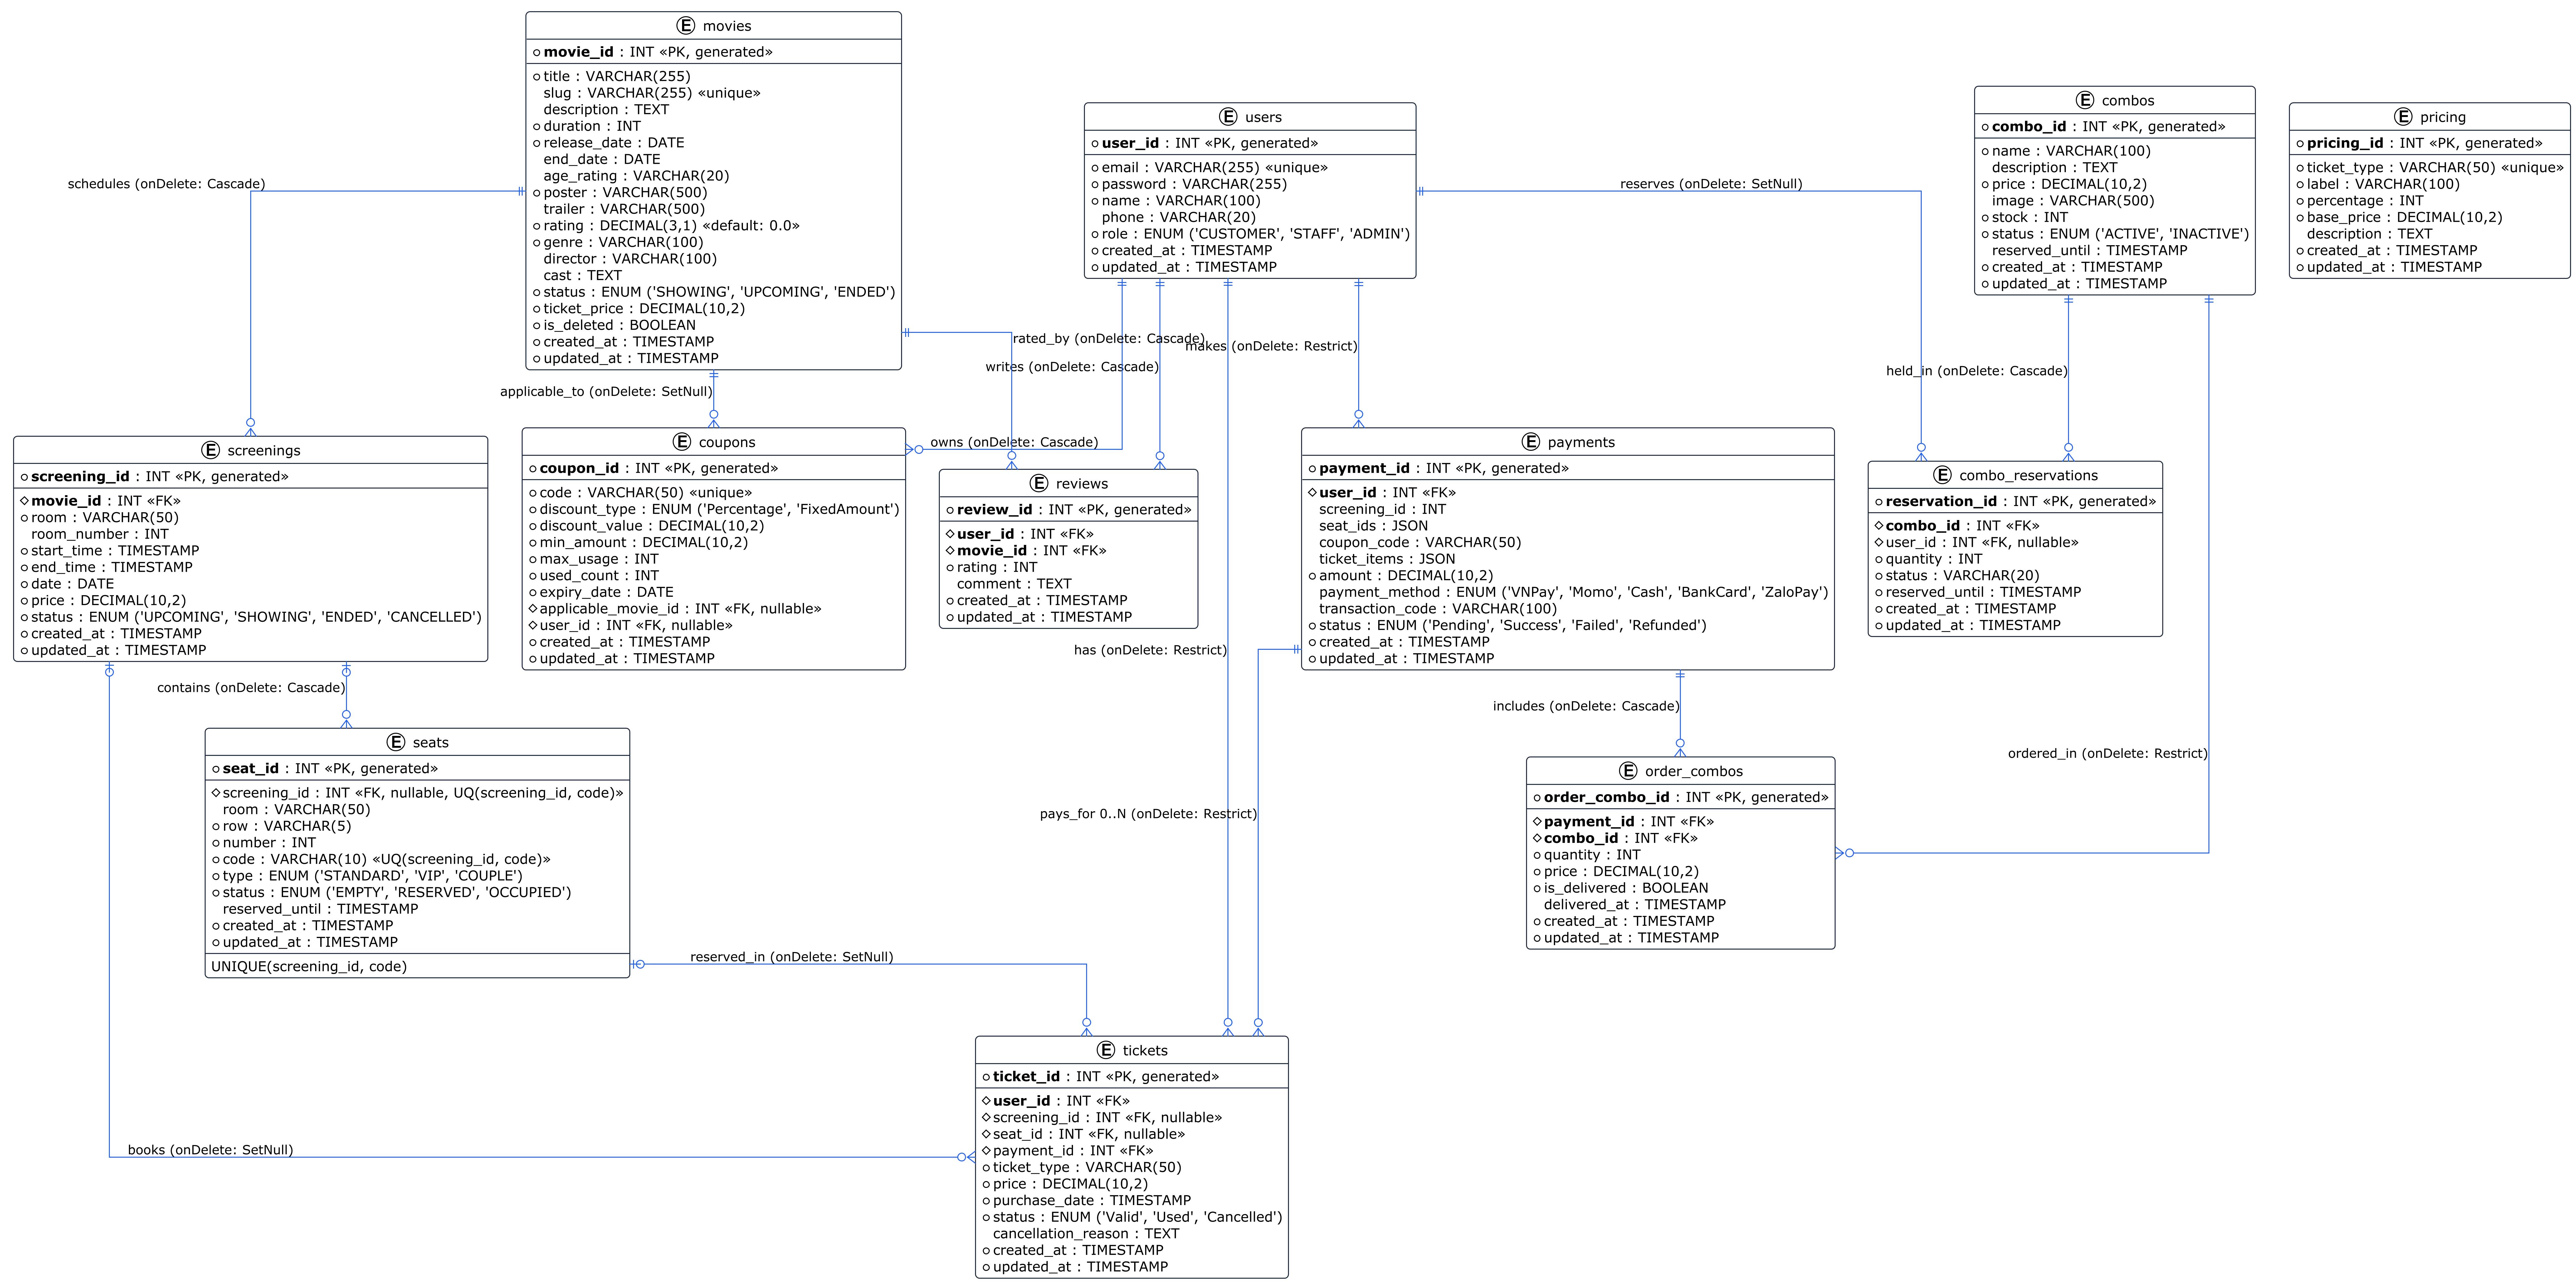
\includegraphics[width=\textwidth,height=0.80\textheight,keepaspectratio]{images/db/ERD_LumiCinema.png}
  \caption{Sơ đồ thực thể kết hợp (ERD) hệ thống LumiCinema}
  \label{fig:erd}
\end{figure}

\begin{figure}[H]
  \centering
  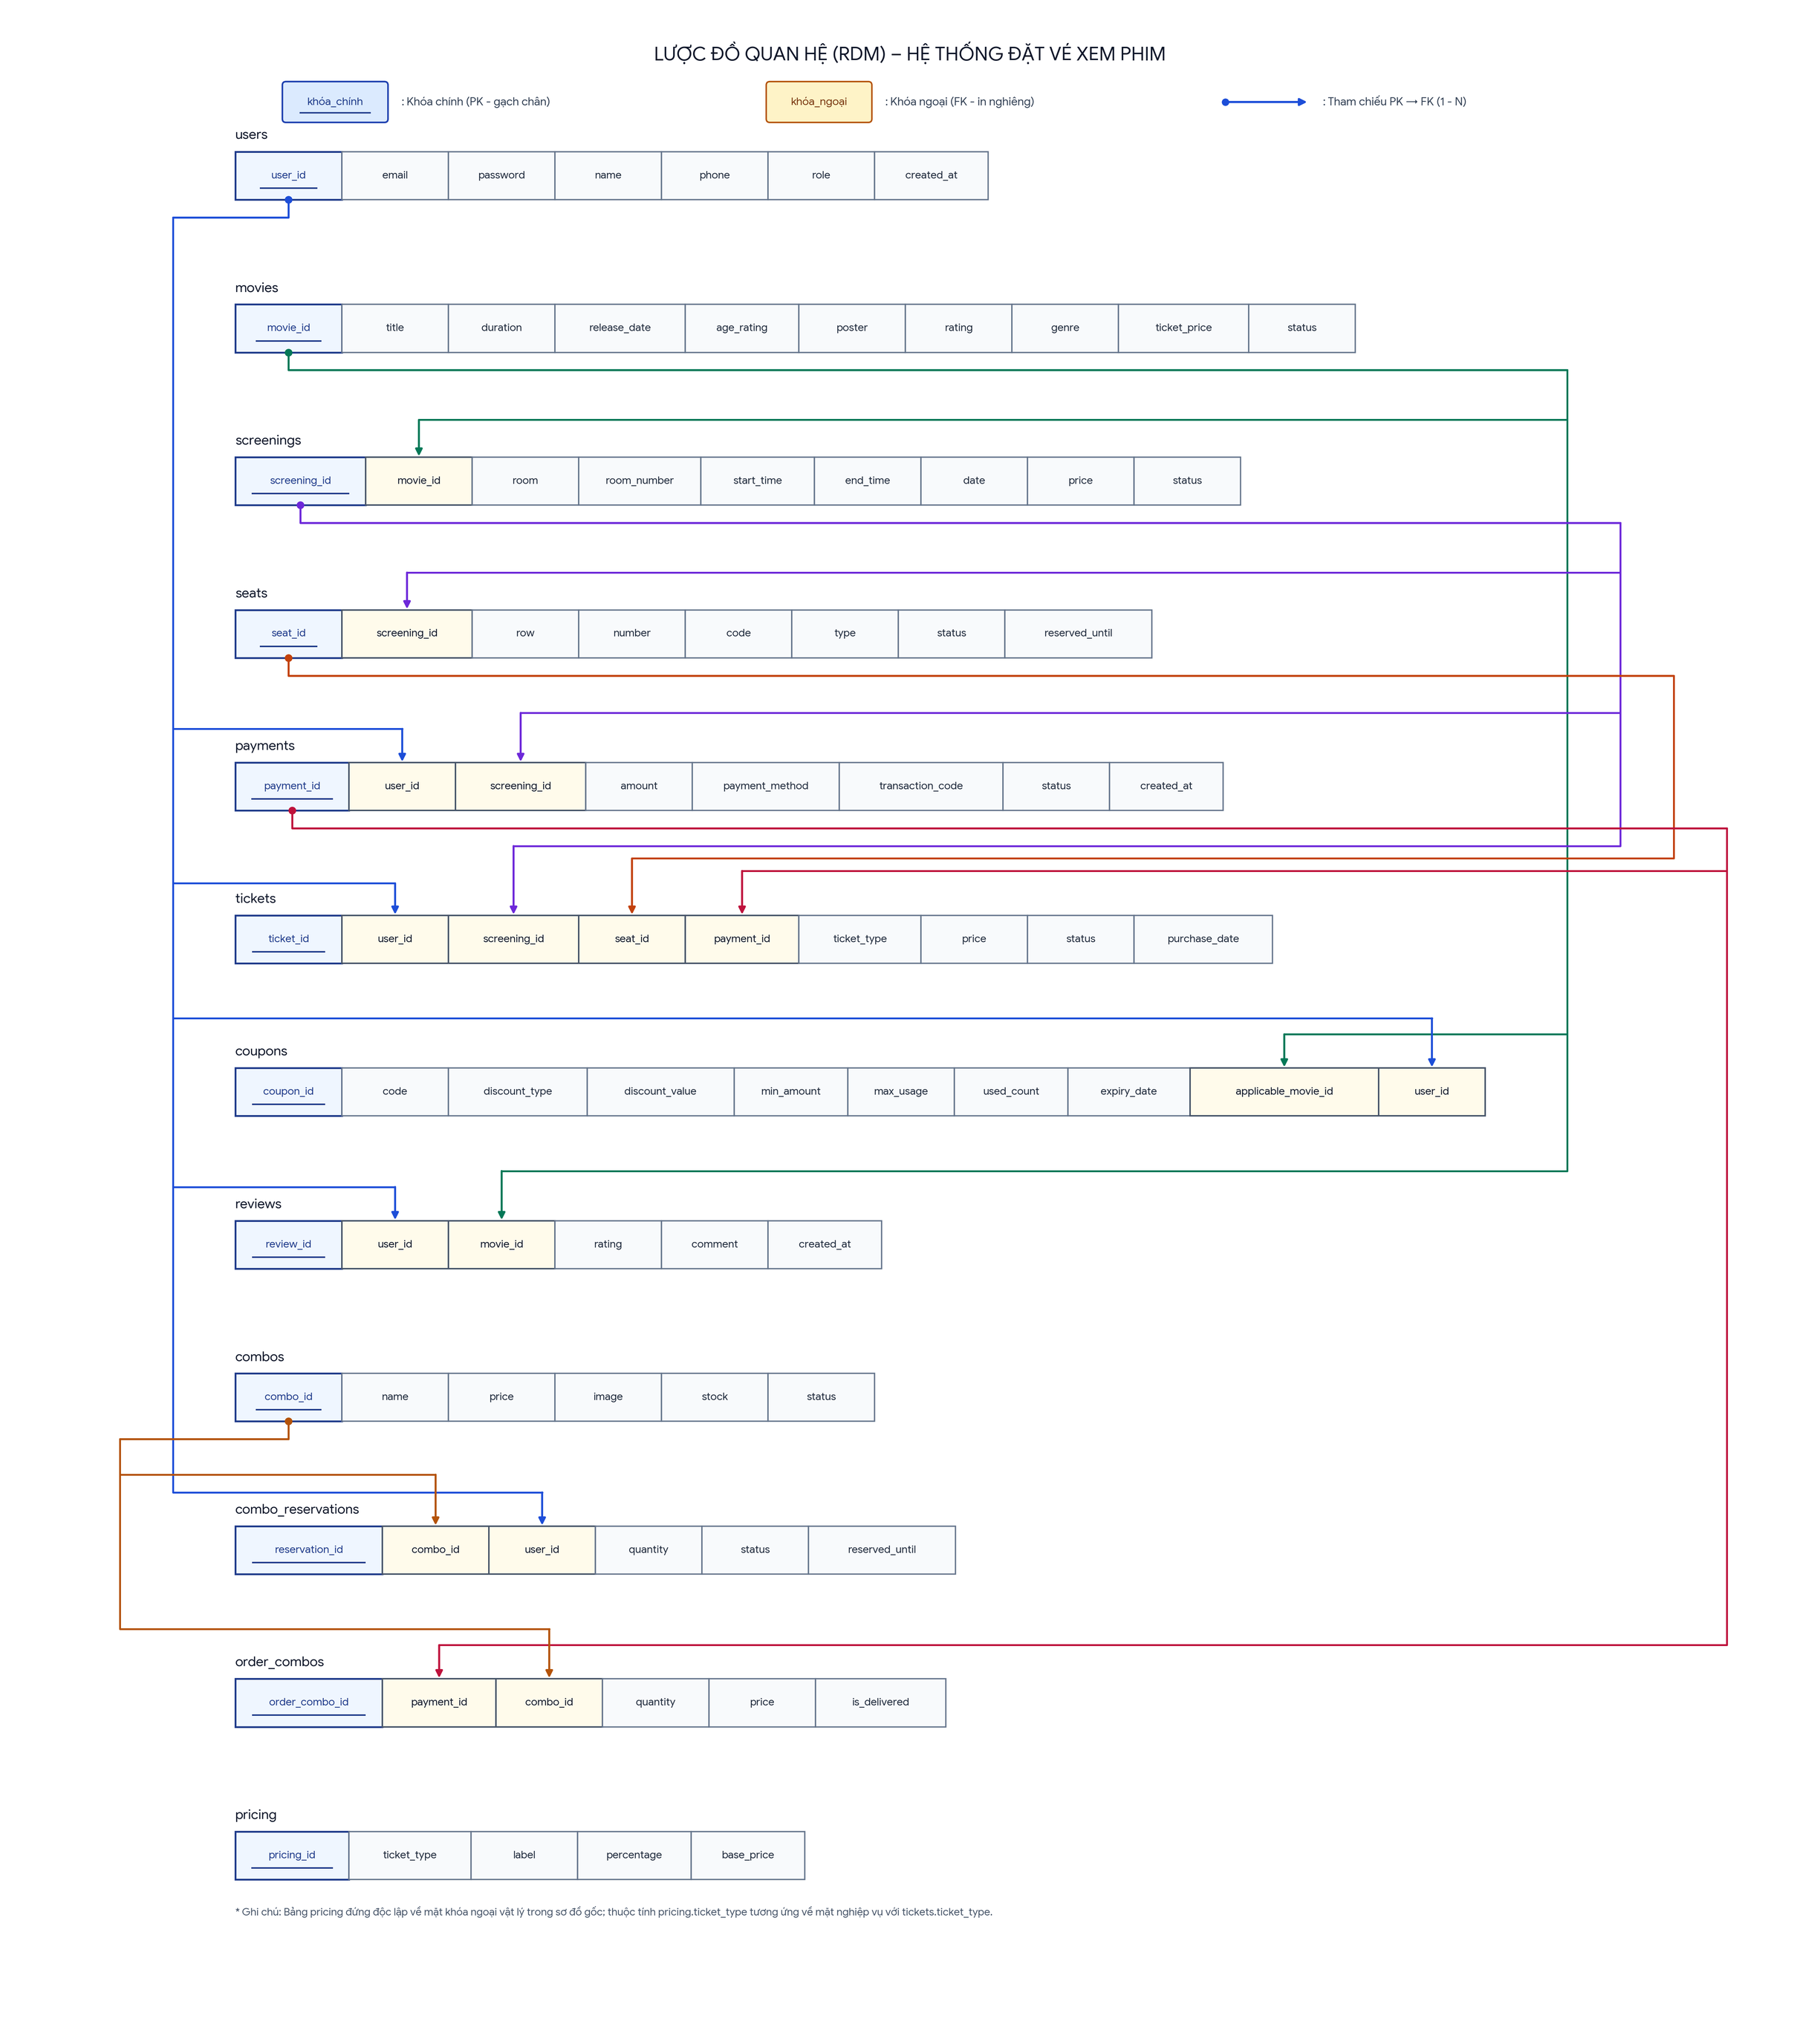
\includegraphics[width=\textwidth,height=0.80\textheight,keepaspectratio]{images/db/rdm_diagram.png}
  \caption{Mô hình dữ liệu quan hệ (RDM) hệ thống LumiCinema}
  \label{fig:rdm}
\end{figure}

\subsection{Danh sách các kiểu liệt kê (Enum)}
\begin{longtable}{|p{4.0cm}|p{11.5cm}|}
\hline
\rowcolor{headerblue} \textbf{Tên Enum} & \textbf{Các giá trị hợp lệ} \\ \hline
\endhead
\textbf{Role} & \texttt{CUSTOMER, STAFF, ADMIN} \\ \hline
\textbf{MovieStatus} & \texttt{SHOWING // Đang chiếu, UPCOMING // Sắp chiếu, ENDED // Ngừng chiếu} \\ \hline
\textbf{ScreeningStatus} & \texttt{UPCOMING, SHOWING, ENDED, CANCELLED} \\ \hline
\textbf{SeatType} & \texttt{STANDARD // Ghế thường, VIP // Ghế VIP, COUPLE // Ghế đôi (Sweetbox)} \\ \hline
\textbf{SeatStatus} & \texttt{EMPTY, RESERVED, OCCUPIED} \\ \hline
\textbf{DiscountType} & \texttt{Percentage // Giảm theo \%, FixedAmount // Giảm theo số tiền cố định} \\ \hline
\textbf{PaymentMethod} & \texttt{VNPay, Momo, Cash, BankCard, ZaloPay} \\ \hline
\textbf{PaymentStatus} & \texttt{Pending // Đang chờ thanh toán, Success // Thanh toán thành công, Failed // Thất bại, Refunded // Đã hoàn tiền} \\ \hline
\textbf{TicketStatus} & \texttt{Valid // Vé hợp lệ, Used // Đã check-in / đã sử dụng, Cancelled // Đã hủy / đã bồi hoàn} \\ \hline
\textbf{ComboStatus} & \texttt{ACTIVE, INACTIVE} \\ \hline
\end{longtable}

\subsection{Mô tả chi tiết 12 bảng dữ liệu}
\subsubsection{Bảng \texttt{User}}
\begin{longtable}{|p{3.6cm}|p{3.0cm}|p{8.9cm}|}
\hline
\rowcolor{headerblue} \textbf{Tên cột} & \textbf{Kiểu dữ liệu} & \textbf{Ràng buộc / Ghi chú} \\ \hline
\endhead
\texttt{id} & \texttt{Int} & \small @id @default(autoincrement()) @map("user\_id") \\ \hline
\texttt{email} & \texttt{String} & \small @unique @db.VarChar(255) \\ \hline
\texttt{password} & \texttt{String} & \small @db.VarChar(255) \\ \hline
\texttt{name} & \texttt{String} & \small @db.VarChar(100) \\ \hline
\texttt{role} & \texttt{Role} & \small @default(CUSTOMER) \\ \hline
\texttt{createdAt} & \texttt{DateTime} & \small @default(now()) @map("created\_at") \\ \hline
\texttt{updatedAt} & \texttt{DateTime} & \small @updatedAt @map("updated\_at") \\ \hline
\end{longtable}

\subsubsection{Bảng \texttt{Movie}}
\begin{longtable}{|p{3.6cm}|p{3.0cm}|p{8.9cm}|}
\hline
\rowcolor{headerblue} \textbf{Tên cột} & \textbf{Kiểu dữ liệu} & \textbf{Ràng buộc / Ghi chú} \\ \hline
\endhead
\texttt{id} & \texttt{Int} & \small @id @default(autoincrement()) @map("movie\_id") \\ \hline
\texttt{title} & \texttt{String} & \small @db.VarChar(255) \\ \hline
\texttt{duration} & \texttt{Int} & \small // Thời lượng (phút) \\ \hline
\texttt{releaseDate} & \texttt{DateTime} & \small @map("release\_date") @db.Date \\ \hline
\texttt{poster} & \texttt{String} & \small @db.VarChar(500) \\ \hline
\texttt{rating} & \texttt{Decimal} & \small @default(0.0) @db.Decimal(3, 1) \\ \hline
\texttt{genre} & \texttt{String} & \small @db.VarChar(100) \\ \hline
\texttt{status} & \texttt{MovieStatus} & \small @default(SHOWING) \\ \hline
\texttt{ticketPrice} & \texttt{Decimal} & \small @default(120000) @map("ticket\_price") @db.Decimal(10, 2) \\ \hline
\texttt{isDeleted} & \texttt{Boolean} & \small @default(false) @map("is\_deleted") \\ \hline
\texttt{createdAt} & \texttt{DateTime} & \small @default(now()) @map("created\_at") \\ \hline
\texttt{updatedAt} & \texttt{DateTime} & \small @updatedAt @map("updated\_at") \\ \hline
\end{longtable}

\subsubsection{Bảng \texttt{Screening}}
\begin{longtable}{|p{3.6cm}|p{3.0cm}|p{8.9cm}|}
\hline
\rowcolor{headerblue} \textbf{Tên cột} & \textbf{Kiểu dữ liệu} & \textbf{Ràng buộc / Ghi chú} \\ \hline
\endhead
\texttt{id} & \texttt{Int} & \small @id @default(autoincrement()) @map("screening\_id") \\ \hline
\texttt{movieId} & \texttt{Int} & \small @map("movie\_id") \\ \hline
\texttt{room} & \texttt{String} & \small @db.VarChar(50) // Vd: "Cinema 01", "Cinema 02" \\ \hline
\texttt{startTime} & \texttt{DateTime} & \small @map("start\_time") \\ \hline
\texttt{endTime} & \texttt{DateTime} & \small @map("end\_time") \\ \hline
\texttt{date} & \texttt{DateTime} & \small @db.Date \\ \hline
\texttt{price} & \texttt{Decimal} & \small @db.Decimal(10, 2) \\ \hline
\texttt{status} & \texttt{ScreeningStatus} & \small @default(UPCOMING) \\ \hline
\texttt{createdAt} & \texttt{DateTime} & \small @default(now()) @map("created\_at") \\ \hline
\texttt{updatedAt} & \texttt{DateTime} & \small @updatedAt @map("updated\_at") \\ \hline
\texttt{movie} & \texttt{Movie} & \small @relation(fields: [movieId], references: [id], onDelete: Cascade) \\ \hline
\end{longtable}

\subsubsection{Bảng \texttt{Seat}}
\begin{longtable}{|p{3.6cm}|p{3.0cm}|p{8.9cm}|}
\hline
\rowcolor{headerblue} \textbf{Tên cột} & \textbf{Kiểu dữ liệu} & \textbf{Ràng buộc / Ghi chú} \\ \hline
\endhead
\texttt{id} & \texttt{Int} & \small @id @default(autoincrement()) @map("seat\_id") \\ \hline
\texttt{row} & \texttt{String} & \small @db.VarChar(5) // Vd: "A", "B", "C" \\ \hline
\texttt{number} & \texttt{Int} & \small // Vd: 1, 2, 3 \\ \hline
\texttt{code} & \texttt{String} & \small @db.VarChar(10) // Vd: "A1", "A2", "C10" \\ \hline
\texttt{type} & \texttt{SeatType} & \small @default(STANDARD) \\ \hline
\texttt{status} & \texttt{SeatStatus} & \small @default(EMPTY) \\ \hline
\texttt{createdAt} & \texttt{DateTime} & \small @default(now()) @map("created\_at") \\ \hline
\texttt{updatedAt} & \texttt{DateTime} & \small @updatedAt @map("updated\_at") \\ \hline
\texttt{screening} & \texttt{Screening?} & \small @relation(fields: [screeningId], references: [id], onDelete: Cascade) \\ \hline
\end{longtable}

\subsubsection{Bảng \texttt{Pricing}}
\begin{longtable}{|p{3.6cm}|p{3.0cm}|p{8.9cm}|}
\hline
\rowcolor{headerblue} \textbf{Tên cột} & \textbf{Kiểu dữ liệu} & \textbf{Ràng buộc / Ghi chú} \\ \hline
\endhead
\texttt{id} & \texttt{Int} & \small @id @default(autoincrement()) @map("pricing\_id") \\ \hline
\texttt{ticketType} & \texttt{String} & \small @unique @map("ticket\_type") @db.VarChar(50) // Vd: "Normal", "Child", "VIP" \\ \hline
\texttt{label} & \texttt{String} & \small @db.VarChar(100) // Vd: "Vé Thường", "Vé Trẻ Em" \\ \hline
\texttt{percentage} & \texttt{Int} & \small @default(100) // \% giá vé: 100\%, 50\%, 180\% \\ \hline
\texttt{basePrice} & \texttt{Decimal} & \small @map("base\_price") @db.Decimal(10, 2) \\ \hline
\texttt{createdAt} & \texttt{DateTime} & \small @default(now()) @map("created\_at") \\ \hline
\texttt{updatedAt} & \texttt{DateTime} & \small @updatedAt @map("updated\_at") \\ \hline
\end{longtable}

\subsubsection{Bảng \texttt{Coupon}}
\begin{longtable}{|p{3.6cm}|p{3.0cm}|p{8.9cm}|}
\hline
\rowcolor{headerblue} \textbf{Tên cột} & \textbf{Kiểu dữ liệu} & \textbf{Ràng buộc / Ghi chú} \\ \hline
\endhead
\texttt{id} & \texttt{Int} & \small @id @default(autoincrement()) @map("coupon\_id") \\ \hline
\texttt{code} & \texttt{String} & \small @unique @db.VarChar(50) \\ \hline
\texttt{discountType} & \texttt{DiscountType} & \small @map("discount\_type") \\ \hline
\texttt{discountValue} & \texttt{Decimal} & \small @map("discount\_value") @db.Decimal(10, 2) \\ \hline
\texttt{minAmount} & \texttt{Decimal} & \small @default(0) @map("min\_amount") @db.Decimal(10, 2) \\ \hline
\texttt{maxUsage} & \texttt{Int} & \small @default(1) @map("max\_usage") \\ \hline
\texttt{usedCount} & \texttt{Int} & \small @default(0) @map("used\_count") \\ \hline
\texttt{expiryDate} & \texttt{DateTime} & \small @map("expiry\_date") @db.Date \\ \hline
\texttt{createdAt} & \texttt{DateTime} & \small @default(now()) @map("created\_at") \\ \hline
\texttt{updatedAt} & \texttt{DateTime} & \small @updatedAt @map("updated\_at") \\ \hline
\texttt{movie} & \texttt{Movie?} & \small @relation(fields: [applicableMovieId], references: [id], onDelete: SetNull) \\ \hline
\texttt{user} & \texttt{User?} & \small @relation(fields: [userId], references: [id], onDelete: Cascade) \\ \hline
\end{longtable}

\subsubsection{Bảng \texttt{Combo}}
\begin{longtable}{|p{3.6cm}|p{3.0cm}|p{8.9cm}|}
\hline
\rowcolor{headerblue} \textbf{Tên cột} & \textbf{Kiểu dữ liệu} & \textbf{Ràng buộc / Ghi chú} \\ \hline
\endhead
\texttt{id} & \texttt{Int} & \small @id @default(autoincrement()) @map("combo\_id") \\ \hline
\texttt{name} & \texttt{String} & \small @db.VarChar(100) \\ \hline
\texttt{price} & \texttt{Decimal} & \small @db.Decimal(10, 2) \\ \hline
\texttt{stock} & \texttt{Int} & \small @default(100) \\ \hline
\texttt{status} & \texttt{ComboStatus} & \small @default(ACTIVE) \\ \hline
\texttt{createdAt} & \texttt{DateTime} & \small @default(now()) @map("created\_at") \\ \hline
\texttt{updatedAt} & \texttt{DateTime} & \small @updatedAt @map("updated\_at") \\ \hline
\end{longtable}

\subsubsection{Bảng \texttt{ComboReservation}}
\begin{longtable}{|p{3.6cm}|p{3.0cm}|p{8.9cm}|}
\hline
\rowcolor{headerblue} \textbf{Tên cột} & \textbf{Kiểu dữ liệu} & \textbf{Ràng buộc / Ghi chú} \\ \hline
\endhead
\texttt{id} & \texttt{Int} & \small @id @default(autoincrement()) @map("reservation\_id") \\ \hline
\texttt{comboId} & \texttt{Int} & \small @map("combo\_id") \\ \hline
\texttt{quantity} & \texttt{Int} & \small @default(1) \\ \hline
\texttt{status} & \texttt{String} & \small @default("RESERVED") @db.VarChar(20) // 'RESERVED' | 'RELEASED' | 'COMPLETED' \\ \hline
\texttt{reservedUntil} & \texttt{DateTime} & \small @map("reserved\_until") \\ \hline
\texttt{createdAt} & \texttt{DateTime} & \small @default(now()) @map("created\_at") \\ \hline
\texttt{updatedAt} & \texttt{DateTime} & \small @updatedAt @map("updated\_at") \\ \hline
\texttt{combo} & \texttt{Combo} & \small @relation(fields: [comboId], references: [id], onDelete: Cascade) \\ \hline
\texttt{user} & \texttt{User?} & \small @relation(fields: [userId], references: [id], onDelete: SetNull) \\ \hline
\end{longtable}

\subsubsection{Bảng \texttt{Payment}}
\begin{longtable}{|p{3.6cm}|p{3.0cm}|p{8.9cm}|}
\hline
\rowcolor{headerblue} \textbf{Tên cột} & \textbf{Kiểu dữ liệu} & \textbf{Ràng buộc / Ghi chú} \\ \hline
\endhead
\texttt{id} & \texttt{Int} & \small @id @default(autoincrement()) @map("payment\_id") \\ \hline
\texttt{userId} & \texttt{Int} & \small @map("user\_id") \\ \hline
\texttt{amount} & \texttt{Decimal} & \small @db.Decimal(10, 2) \\ \hline
\texttt{status} & \texttt{PaymentStatus} & \small @default(Pending) \\ \hline
\texttt{createdAt} & \texttt{DateTime} & \small @default(now()) @map("created\_at") \\ \hline
\texttt{updatedAt} & \texttt{DateTime} & \small @updatedAt @map("updated\_at") \\ \hline
\texttt{user} & \texttt{User} & \small @relation(fields: [userId], references: [id], onDelete: Restrict) \\ \hline
\end{longtable}

\subsubsection{Bảng \texttt{Ticket}}
\begin{longtable}{|p{3.6cm}|p{3.0cm}|p{8.9cm}|}
\hline
\rowcolor{headerblue} \textbf{Tên cột} & \textbf{Kiểu dữ liệu} & \textbf{Ràng buộc / Ghi chú} \\ \hline
\endhead
\texttt{id} & \texttt{Int} & \small @id @default(autoincrement()) @map("ticket\_id") \\ \hline
\texttt{userId} & \texttt{Int} & \small @map("user\_id") \\ \hline
\texttt{paymentId} & \texttt{Int} & \small @map("payment\_id") \\ \hline
\texttt{ticketType} & \texttt{String} & \small @map("ticket\_type") @db.VarChar(50) \\ \hline
\texttt{price} & \texttt{Decimal} & \small @db.Decimal(10, 2) \\ \hline
\texttt{purchaseDate} & \texttt{DateTime} & \small @default(now()) @map("purchase\_date") \\ \hline
\texttt{status} & \texttt{TicketStatus} & \small @default(Valid) \\ \hline
\texttt{createdAt} & \texttt{DateTime} & \small @default(now()) @map("created\_at") \\ \hline
\texttt{updatedAt} & \texttt{DateTime} & \small @updatedAt @map("updated\_at") \\ \hline
\texttt{user} & \texttt{User} & \small @relation(fields: [userId], references: [id], onDelete: Restrict) \\ \hline
\texttt{screening} & \texttt{Screening?} & \small @relation(fields: [screeningId], references: [id], onDelete: SetNull) \\ \hline
\texttt{seat} & \texttt{Seat?} & \small @relation(fields: [seatId], references: [id], onDelete: SetNull) \\ \hline
\texttt{payment} & \texttt{Payment} & \small @relation(fields: [paymentId], references: [id], onDelete: Restrict) \\ \hline
\end{longtable}

\subsubsection{Bảng \texttt{OrderCombo}}
\begin{longtable}{|p{3.6cm}|p{3.0cm}|p{8.9cm}|}
\hline
\rowcolor{headerblue} \textbf{Tên cột} & \textbf{Kiểu dữ liệu} & \textbf{Ràng buộc / Ghi chú} \\ \hline
\endhead
\texttt{id} & \texttt{Int} & \small @id @default(autoincrement()) @map("order\_combo\_id") \\ \hline
\texttt{paymentId} & \texttt{Int} & \small @map("payment\_id") \\ \hline
\texttt{comboId} & \texttt{Int} & \small @map("combo\_id") \\ \hline
\texttt{quantity} & \texttt{Int} & \small Thuộc tính dữ liệu \\ \hline
\texttt{price} & \texttt{Decimal} & \small @db.Decimal(10, 2) // Giá combo tại thời điểm mua \\ \hline
\texttt{isDelivered} & \texttt{Boolean} & \small @default(false) @map("is\_delivered") \\ \hline
\texttt{createdAt} & \texttt{DateTime} & \small @default(now()) @map("created\_at") \\ \hline
\texttt{updatedAt} & \texttt{DateTime} & \small @updatedAt @map("updated\_at") \\ \hline
\texttt{payment} & \texttt{Payment} & \small @relation(fields: [paymentId], references: [id], onDelete: Cascade) \\ \hline
\texttt{combo} & \texttt{Combo} & \small @relation(fields: [comboId], references: [id], onDelete: Restrict) \\ \hline
\end{longtable}

\subsubsection{Bảng \texttt{Review}}
\begin{longtable}{|p{3.6cm}|p{3.0cm}|p{8.9cm}|}
\hline
\rowcolor{headerblue} \textbf{Tên cột} & \textbf{Kiểu dữ liệu} & \textbf{Ràng buộc / Ghi chú} \\ \hline
\endhead
\texttt{id} & \texttt{Int} & \small @id @default(autoincrement()) @map("review\_id") \\ \hline
\texttt{userId} & \texttt{Int} & \small @map("user\_id") \\ \hline
\texttt{movieId} & \texttt{Int} & \small @map("movie\_id") \\ \hline
\texttt{rating} & \texttt{Int} & \small // 1 đến 5 sao \\ \hline
\texttt{createdAt} & \texttt{DateTime} & \small @default(now()) @map("created\_at") \\ \hline
\texttt{updatedAt} & \texttt{DateTime} & \small @updatedAt @map("updated\_at") \\ \hline
\texttt{user} & \texttt{User} & \small @relation(fields: [userId], references: [id], onDelete: Cascade) \\ \hline
\texttt{movie} & \texttt{Movie} & \small @relation(fields: [movieId], references: [id], onDelete: Cascade) \\ \hline
\end{longtable}

